\afuncT{invclip}{Inverse Clip}{selectionOperations}
\\\cvsiplh
\afh
{
\ttfamily
\\\hspace*{.04\textwidth}
\begin{tabular}{l}
void vsip\_minvclip\_d(\\*\hspace*{1cm}const vsip\_mview\_d*, vsip\_scalar\_d, vsip\_scalar\_d,\\*\hspace*{1cm}vsip\_scalar\_d, vsip\_scalar\_d, vsip\_scalar\_d, const vsip\_mview\_d*);\\
void vsip\_minvclip\_f(\\*\hspace*{1cm}const vsip\_mview\_f*, vsip\_scalar\_f, vsip\_scalar\_f,\\*\hspace*{1cm}vsip\_scalar\_f, vsip\_scalar\_f, vsip\_scalar\_f, const vsip\_mview\_f*);\\
void vsip\_vinvclip\_d(\\*\hspace*{1cm}const vsip\_vview\_d*, vsip\_scalar\_d, vsip\_scalar\_d,\\*\hspace*{1cm}vsip\_scalar\_d, vsip\_scalar\_d, vsip\_scalar\_d, const vsip\_vview\_d*);\\
void vsip\_vinvclip\_f(\\*\hspace*{1cm}const vsip\_vview\_f*, vsip\_scalar\_f, vsip\_scalar\_f,\\*\hspace*{1cm}vsip\_scalar\_f, vsip\_scalar\_f, vsip\_scalar\_f, const vsip\_vview\_f*);\\
void vsip\_vinvclip\_i(\\*\hspace*{1cm}const vsip\_vview\_i*, vsip\_scalar\_i, vsip\_scalar\_i,\\*\hspace*{1cm}vsip\_scalar\_i, vsip\_scalar\_i, vsip\_scalar\_i, const vsip\_vview\_i*);\\
void vsip\_vinvclip\_si(\\*\hspace*{1cm}const vsip\_vview\_si*, vsip\_scalar\_si, vsip\_scalar\_si,\\*\hspace*{1cm}vsip\_scalar\_si, vsip\_scalar\_si, vsip\_scalar\_si, const vsip\_vview\_si*);\\
void vsip\_vinvclip\_uc(\\*\hspace*{1cm}const vsip\_vview\_uc*, vsip\_scalar\_uc, vsip\_scalar\_uc,\\*\hspace*{1cm}vsip\_scalar\_uc, vsip\_scalar\_uc, vsip\_scalar\_uc, const vsip\_vview\_uc*);\\
\end{tabular}
}
\pyjvsiph
\viewmthd{No}{NA}{NA}{NA}
\apyfunc{Yes}{\ttbf{invclip(in,t1,t2,t3,c1,c2,out)}}
\inputminted[linenos=true,resetmargins=true,xleftmargin=.11\textwidth,fontfamily=tt,fontsize=\small]{python}{./pyJvsip_examples/eXinvclip.py}
\hspace*{.08\textwidth}{\rmfamily For result see figure \ref{fig:invClipExample}.}\\
\begin{minipage}[c]{\textwidth}\centering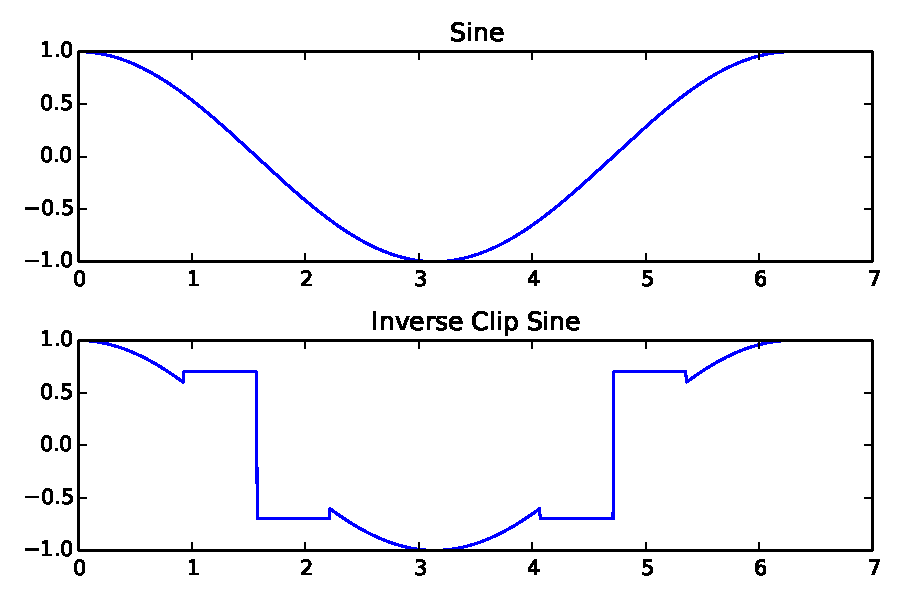
\includegraphics[width=0.8\textwidth]{./pyJvsip_examples/eXinvclip}\captionof{figure}{Inverse Clip Example}
\label{fig:invClipExample}\end{minipage}
\pyComment{
\item{The clip function works much the same as \cvl{} except the output is returned.}
\item{In line 6 of the example we used the \ttbf{empty} method to create the output 
vector and saved a reference in the left value.}
\item{The \ttbf{invclip} function is complicated. See the \cvl{} specification for more complete details.}
\item{The \ttbf{view} \ttbf{in} is clipped according to the rules of the function. The clipping checks are set by \ttbf{t1} (low),  \ttbf{t2}(mid), and \ttbf{t3}(high); and the clip values are set by \ttbf{c1} and \ttbf{c2} accordingly.}
\item{If \ttbf{in==out} then the function is done in-place}
}